\documentclass[a4paper,12pt]{extarticle}
\usepackage{geometry}
\usepackage[T1]{fontenc}
\usepackage[utf8]{inputenc}
\usepackage[english,russian]{babel}
\usepackage{amsmath}
\usepackage{amsthm}
\usepackage{amssymb}
\usepackage{fancyhdr}
\usepackage{setspace}
\usepackage{graphicx}
\usepackage{colortbl}
\usepackage{tikz}
\usepackage{pgf}
\usepackage{subcaption}
\usepackage{listings}
\usepackage{indentfirst}
\usepackage{float}

\usepackage[
backend=biber,
style=numeric,
maxbibnames=99
]{biblatex}
\addbibresource{refs.bib}

\usepackage[colorlinks,citecolor=blue,linkcolor=blue,bookmarks=false,hypertexnames=true, urlcolor=blue]{hyperref} 
\usepackage{indentfirst}
\usepackage{mathtools}
\usepackage{booktabs}
\usepackage[flushleft]{threeparttable}
\usepackage{tablefootnote}

\usepackage{chngcntr} % нумерация графиков и таблиц по секциям
\counterwithin{table}{section}
\counterwithin{figure}{section}

\graphicspath{{graphics/}}%путь к рисункам

\makeatletter
% \renewcommand{\@biblabel}[1]{#1.} % Заменяем библиографию с квадратных скобок на точку
\makeatother

\geometry{left=2.5cm}% левое поле
\geometry{right=1.0cm}% правое поле
\geometry{top=2.0cm}% верхнее поле
\geometry{bottom=2.0cm}% нижнее поле
\setlength{\parindent}{1.25cm}
\renewcommand{\baselinestretch}{1.5} % междустрочный интервал


\newcommand{\bibref}[3]{\hyperlink{#1}{#2 (#3)}} % biblabel, authors, year
\addto\captionsrussian{\def\refname{Список литературы}} 

\renewcommand{\theenumi}{\arabic{enumi}}
\renewcommand{\labelenumi}{\arabic{enumi}}
\renewcommand{\theenumii}{.\arabic{enumii}}
\renewcommand{\labelenumii}{\arabic{enumi}.\arabic{enumii}.}
\renewcommand{\theenumiii}{.\arabic{enumiii}}
\renewcommand{\labelenumiii}{\arabic{enumi}.\arabic{enumii}.\arabic{enumiii}.}

\begin{document}
\input{title_kr} % титульный лист 
\newpage
\setcounter{page}{2}

{
	\hypersetup{linkcolor=black}
	\tableofcontents
}

\newpage

\section*{Аннотация}
Цель проекта создать колоночный формат и реализовать колоночный движок, который
будет успешно проходить бенчмарк ClickBench.

\addcontentsline{toc}{section}{Аннотация}

\section*{Ключевые слова}
Колоночный движок, колоночный формат, базы данных, ClickBench, pull, columnar engine.
\pagebreak

\section{Введение}
\subsection{Описание предметной области}
СУБД (Системы Управления Базами Данных) являются неотъемлемой частью любого крупного
сервиса. Они позволяют эффективно хранить и обрабатывать огромные объемы данных,
отвечая на SQL запросы агрегаций, группировок, фильтраций и других операций.

В частности, колоночные движки являются популярным решением для исполнения SQL
запросов к таблицам, которые не требуют функционала добавления/удаления строк.
У них есть свой колоночный формат(данные лежат столбцами, а не строками), что
минимизирует количество cache miss’ов (промахов по кэшу 
процессора, что влечет загрузку новых кэш-линий в процессор),
 на 
запросах, использующих малую часть колонок и чтений
с диска при ответе на запрос. Благодаря этому колоночные движки могут быть в разы
эффективнее, чем строковые движки при ответе на запросы, которые обращаются лишь к
паре столбцов.



Для оценки производительности движков используем ClickBench. Этот способ позволяет
оценить эффективность аналитических движков, бенчмарк прогоняет запросы на таблице, которая
содержит порядка 100 столбцов и около 90 миллионов строк, при этом все данные
анонимизированы и основаны на работе популярного сервиса, что делает условия
максимально приближенными к реальным.

\subsection{Постановка задачи}
Переложить данные, в свой колоночный формат и реализовать колоночный движок,
работающий с новым форматом, который сможет
успешно проходить бенчмарк ClickBench.

\subsection{Структура работы}
Колоночный формат:
класс для чтения и записи csv файла, а также разработан
колоночный формат и класс для чтения и записи bzn формата.

Легко масштабируемый движок, построенный на pull архитектуре.
Благодаря простым интерфейсам операторов,
выражений и агрегаций движок является очень гибким и добавление нового функционала не
составит труда.

Исходный код проекта\cite{GitHub}.


\section{Обзор литературы}
\subsection{ClickBench}
ClickBench \cite{clickbench} -- это инструмент, который позволяет протестировать
производительность БД на базовой нагрузке сфер бизнес аналитики и дашбордов
реального времени. Универсальный бенчмарк, который используя самые базовые
операции в запросах оценивает эффективность СУБД.

Данные представляют собой фактическую запись трафика из одной из крупнейшей в мире
платформы в сфере веб-аналитики. Они анонимны и лежат в виде одной плоской таблицы
на 99 997 497 строк и 105 столбцов. Всего в бенчмарке 43 SQL запроса, они
представляют собой: базовые агрегации, группировки, сортировки+limit, а также
тяжелые запросы. При прогоне запросов запрещено кеширование, каждый запрос
прогоняется три раза.

Целью является прохождение бенчмарка ClickBench,
лидеры по производительности расположены на сайте бенчмарка \cite{clickbench}. Результаты
запуском на сайте представлены на различных машинах, как с cold (запуск на свежей
машине), так и warm (запуск с прогретыми под нашу задачу кешами и процессором)
режимами. Выберем тройку лидеров (все они являются колоночными).
ClickHouse \cite{clickhouse}, Parquet \cite{parquet} и DuckDB \cite{duckdb}.
Выделим особенности каждого из движков.

\subsection{Колоночные движки}

ClickHouse \cite{clickhouse} использует собственные форматы хранения (семейство
движков MergeTree), сжатие и векторные инструкции процессора для обработки данных.

DuckDB \cite{duckdb} — это встраиваемая (in-process) база данных. У неё нет сервера,
она работает внутри процесса и имеет хорошую совместимость, что и есть ее главные особенности.

Parquet \cite{parquet} — это колоночный формат хранения данных, который содержит
метаданные (статистику min/max), что позволяет движкам читать только нужные части
файла.

У всех трёх движков есть свои особенности, которые позволяют им быть
производительными.

\subsection{Основные понятия и определения}
Введем определение batch’a. Скажем, что количество колонок в нашей таблице это $m$.
batch — это часть таблицы, которая помещается в оперативную память.
Данные столбцов лежат рядом друг с другом. На это можно смотреть так: возьмем $k$
подряд идущих строк таблицы, транспонируем их и наш batch готов. То есть вся
исходная таблица представима в виде $batch_1 \sqcup batch_2 \sqcup \dots \sqcup batch_k$,
где $k$ — количество batch’ей, зависящее от количества строк в таблице и размера
batch’a (на данный момент размер определяется как количество, хранящихся в batch’e).
Для наглядной картинки можно обратиться к формату файла движка
Apache Parquet \cite{parquet}. У них batch — это row group (chunk).

Стоит ознакомиться с SQL синтаксисом, запросы исполняемые движком лежат в 
репозитории проекта \cite{GitHub}, файл queries.sql, осознание того
что делают эти запросы будет очень
хорошим пререквизитом для полного понимания структуры работы.

Pull-based подход -- это архитектура, в которой каждому оператору
не важно какой оператор на входе и какой оператор на выходе. Все что есть у
операторов для взаимодействия друг с другом это метод \texttt{Next}, который прокидывает
батчи между операторами, пока есть что прокидывать. В качестве примера
рассмотрим задачу: нужно найти количество строк в таблице с непустой строкой в колонке $j$.
В таком случае это последовательность операторов \texttt{scan} $\rightarrow$ \texttt{filter} $\rightarrow$
\texttt{aggregate}.
Для результата нужно позвать \texttt{Next} от aggregate, он в свою очередь
будет звать \texttt{Next} от \texttt{filter} пока не закончатся данные, \texttt{filter} зовет
\texttt{Next} от \texttt{scan}, \texttt{scan} дает батч, \texttt{filter} оставляет только строки с непустой строкой в колонке
$j$, дает батч \texttt{aggregate}'у, тот в свою очередь накапливает количество строк
в батчах, которые дает \texttt{filter} и возвращает ответ. Похожий метод используется в статье
\cite{pull_volcano}, в которой также есть pull модель, но более сильная в плане параллелизации.

Определим выражение. Это какая-то последовательность действий с колонками,
 выстраивающихся в Abstract Syntax Tree. Для осознания того, что такое AST,
можно посмотреть на построение дерева для польской записи математических выражений,
или разобраться в устройстве LISP языка. Листовыми выражениями будем называть
ссылку на колонку или литерал, подробнее в описании структуры.

План запросов -- это композиция операторов и выражений над колонками,
которая нацелена на исполнение конкретного sql запроса.

Парсер -- это программа, которая занимается построением плана запросов по sql запросов.


\section{Описание предлагаемого метода}


\begin{figure}[H]
    \centering
    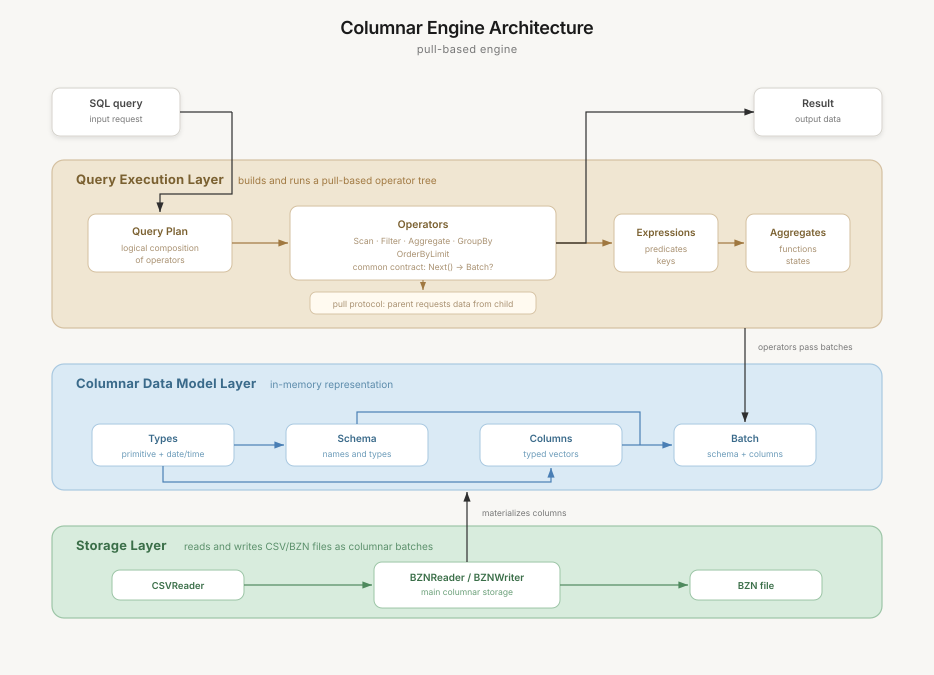
\includegraphics[width=0.8\textwidth]{architecture.pdf}
    \caption{Архитектура проекта Columnar Engine.}
    \label{fig:architecture}
\end{figure}


\subsection{Структура input output логики}

\begin{itemize}
\item \texttt{rwconsts.h} - файл, содержащий константы для размера батча, разделителей 
строк в метаданных.

\item \texttt{types.h} - реализация логики типов, конвертация между типами,
cpp тип по enum типу.

\item \texttt{datatype.h} - логика работы с датами. Описано в разделе о bzn формате.

\item \texttt{class Schema} — содержит информацию о названиях и типах столбцов таблицы.

\item \texttt{class Column} — содержит данные одного столбца таблицы, представляет из себя
\texttt{std::vari}-\texttt{ant<std::vector<type\_1>, \dots>} имеет метод \texttt{TranslateTo}, который
переводит колонку из одного типа в другой.

\item \texttt{class Batch} — batch, определенный ранее, хранит данные как \texttt{std::vector<Column>} и
держит рядом класс \texttt{Schema}, это сделано для того чтобы в батч можно было подставить
другую схему, что вызовет трансформацию столбцов (\texttt{TranslateTo}) в нужные типы.

\item \texttt{class CSV-Reader} — читает csv файл согласно RFC-4180 \cite{rfc4180} и возвращает
batch строкового типа.

\item \texttt{class CSV-Writer} — принимает batch, дает ему новую схему в которой типы это строка,
данные в батче переводятся в строки, записываем в csv файл согласно
RFC-4180 \cite{rfc4180}.

\item \texttt{class BZN-Reader}— читает колоночный формат и возвращает batch.
В конструкторе принимает множество колонок, которые нужно читать, при передаче
пустого списка читает все колонки.

\item \texttt{class BZN-Writer} — принимает batch и записывает в колоночный формат (при
инициализации создает массив с разметкой батчей, который заполняется по ходу записи).

\end{itemize}
Для чтения пользуемся \texttt{fstream} так как это достаточно простой и понятный метод.
В случае csv читаем побайтово, в случае с bzn читаем все кроме строк сразу блоком,
строки по специфике хранения читаем побайтово. Сделать \texttt{mmap} файла потребовало бы 
более тяжелой логики и могло дать хороший рост производительности в io части,
но такой эксперимент потребовал бы много времени.

\subsection{Колоночный формат bzn и логика типов в классе Column}
Поддерживаются следующие типы данных:
\texttt{bool}, \texttt{int16\_t}, \texttt{int32\_t}, \texttt{int64\_t},
\texttt{double}, \texttt{long double}, \texttt{string}, \texttt{date}, \texttt{timestamp}.

\begin{itemize}
    \item \texttt{bool}:
  Не храним явно на диске, этот тип колонки используется только на этапе вычисления выражений с колонками.
    \item \texttt{int16\_t}, \texttt{int32\_t}, \texttt{int64\_t}:
    \begin{itemize}
        \item \texttt{csv $\rightarrow$ bzn} : \texttt{std::from\_chars} от строкового представления числа в \texttt{int\_(16|32|64)\_t} так как работает быстрее, чем \texttt{std::stoll}, кладем побайтово \texttt{sizeof} байт в little-endian формате.
        \item \texttt{bzn $\rightarrow$ csv} : \texttt{std::to\_string} целого числа.
    \end{itemize}
    \item \texttt{double}:
    \begin{itemize}
        \item \texttt{csv $\rightarrow$ bzn} : \texttt{std::from\_chars} от строкового представления числа в \texttt{double}, далее \texttt{memcpy} \texttt{sizeof(double)} байт.
        \item \texttt{bzn $\rightarrow$ csv} : \texttt{std::to\_string} вещественного числа.
    \end{itemize}
    \item \texttt{\texttt{long double}}:
    \begin{itemize}
        \item \texttt{csv $\rightarrow$ bzn} : \texttt{std::stold} так как \texttt{std::from\_chars}
        в силу зависимости от системы не поддерживается, кладем в \texttt{long double}, далее \texttt{memcpy} \texttt{sizeof} байт.
        \item \texttt{bzn $\rightarrow$ csv} : \texttt{std::to\_string} вещественного числа.
    \end{itemize}

    \item \texttt{\texttt{string}}:
    \begin{itemize}
        \item \texttt{csv $\rightarrow$ bzn} :
Записывается как последовательность байт(символов), описывающая нашу строку, после
чего идет \texttt{'\textbackslash x1F'} — специальный символ, демонстрирующий конец
строки.
        \item \texttt{bzn $\rightarrow$ csv} : читаем до \texttt{'\textbackslash x1F'} и записываем строку в csv.

	\end{itemize}
    \item \texttt{date}:
    Храним количество дней(в нашей системе координат, особенности которой в следующем абзаце)
     c 1970.01.01 в \texttt{int32\_t}.

    В году 512 дней, в месяце 32 дня, потому что в нашей задаче для дат
	требуется только сравнение и транслирование yyyy-mm-dd $\leftrightarrow$ \texttt{int32\_t},
	очевидно, что порядок в таком случае сохраняется,
	но теряются операции сложения и вычитания, что можно компенсировать обычными
    методом конвертирования.
	
	Этот подход позволил тратить меньше чем встроенные парсеры, и чем свой ранее написанный
	парсер, который хранил префиксные суммы дней в зависимости от года от 1970 года, потому что
    теперь все деления и нетривиальные операции заменяются быстрыми операциями со степенями двойки.
    \begin{itemize}
        \item \texttt{csv $\rightarrow$ bzn} : \texttt{std::from\_chars} от $yyyy, mm, dd$, далее $yyyy * 512 + mm * 32 + dd \rightarrow$ \texttt{int32\_t}.
        \item \texttt{bzn $\rightarrow$ csv} : обратная процедура с \texttt{std::to\_string}.
    \end{itemize}


    \item \texttt{timestamp}:
    Храним количество секунд c 1970.01.01-00:00:00 в \texttt{int64\_t}.

    \begin{itemize}
        \item \texttt{csv $\rightarrow$ bzn} : получаем дни $dd$ от \texttt{data}, далее \texttt{std::from\_chars} от $hh,mm,ss$, далее $dd * 24 * 3600 + hh * 3600 + mm * 60 + ss \rightarrow$ \texttt{int64\_t}.
        \item \texttt{bzn $\rightarrow$ csv} : обратная процедура с \texttt{std::to\_string}.
    \end{itemize}
\end{itemize}


\begin{figure}[ht]
    \centering
    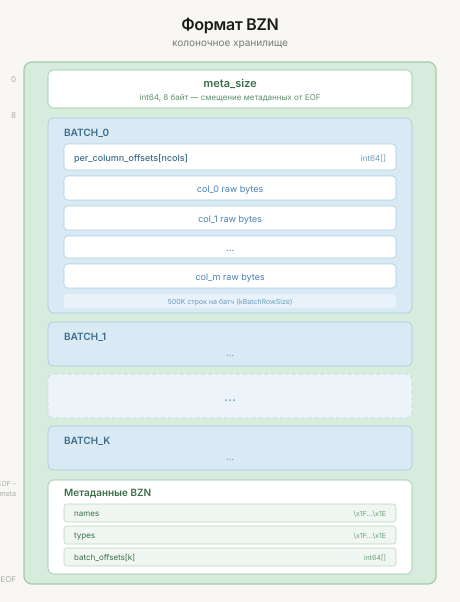
\includegraphics[width=0.5\textwidth]{bzn-format.pdf}
    \caption{Схема хранения файла.}
    \label{fig:file_schema}
\end{figure}

batch в bzn формате лежит как: 
\begin{equation}
    \left[ \text{метаданные} \right] 
    \left[ \text{данные} \right]
\end{equation}
Метаданные хранятся как подряд
идущие \texttt{int64\_t}, которые описывают позиции в файле, с которых начинается
каждая колонка $poscolumn_1, poscolumn_2, \dots, poscolumn_m$. После метаинформации
лежат сами данные колонок, с позиции $poscolumn_i$ в файле лежит $i$-ая колонка (о том
как хранятся различные типы уже говорили). Далее поговорим о метаданных всего файла.
Из которых будет очевидно количество колонок в таблице, а значит и задача чтения 
батча очевидна.

Формат bzn выглядит следующим образом, $batch_i$ хранится как сказано выше:
\begin{equation}
    \left[ \text{размер метаданных} \right] 
     \left[ \text{batch}_1 \right] 
     \left[ \text{batch}_2 \right] 
    \cdots 
    \left[ \text{batch}_k \right] 
    \left[ \text{метаданные} \right]
\end{equation}

Метаданные в конце файла хранятся как:
\begin{equation}
    \left[ \text{имена столбцов} \right] 
    \left[ \text{типы столбцов} \right] 
    \left[ \text{разметка батчей} \right]
\end{equation}

Где имена столбцов — это последовательность строк, разделенных символом
\texttt{'\textbackslash x1F'}, после которых идет символ \texttt{'\textbackslash x1E'},
говорящий об окончании этой секции метаданных. Типы столбцов хранятся аналогично их
строковыми представлениями. После них также идет символ \texttt{'\textbackslash x1E'}
и начинается разметка батчей, которая представляет собой последовательность
\texttt{int64\_t}, каждый из которых говорит о позиции в файле, с которой начинается
соответствующий батч.


\subsection{Логика исполнения запросов}
Логика исполнения запросов нацелена на простое построение плана.
Для пользователя созданы
базовые интерфейсы агрегаций, выражений над колонками и операторов,
которые позволяют без проблем добавить новый функционал и построить план
исполнения запроса.
Для добавления нового функционала, его нужно унаследовать от базового класса 
с интерфейсами и написать собственную реализацию нового метода.

\subsubsection{Агрегации}
Базовый интерфейс \texttt{IAggregateFunc}, агрегации, унаследованные от этого класса,
должны переопределить методы:

\begin{itemize}
    \item \texttt{std::shared\_ptr<IAggregateState> CreateState()} : создание пустого
    состояния агрегации.
    \item \texttt{void Update(std::shared\_ptr<IAggregateState>, const Column\&)} :
    обновление состояния по очередному батчу значений.
    \item \texttt{Column Finalize(std::shared\_ptr<IAggregateState>)} : получение итоговой
    колонки из одного элемента.
\end{itemize}

Состояние агрегации отделено от самой функции агрегации. Это позволяет одному объекту
агрегации создавать разные независимые состояния для разных групп в операторе
\texttt{GroupByOperator}: для каждого ключа группировки хранится свой
\texttt{IAggregateState}, а при поступлении нового батча соответствующее состояние
пересчитывается методом \texttt{Update}. После обработки всех батчей метод
\texttt{Finalize} превращает накопленное состояние в одноэлементную колонку результата.
Для создания state нужно определить деструктор и поля которые будут в нем лежать.

Поддерживаемые агрегации:

\begin{itemize}
    \item \texttt{CountFunc} : считает количество строк во входной колонке. В состоянии
    \texttt{CountState} хранится одно поле \texttt{size\_t res} --- текущее количество
    элементов. При пересчете состояние увеличивается на \texttt{col.GetSize()}.
    В \texttt{Finalize} возвращается колонка типа \texttt{int32\_t} из одного элемента,
    равного накопленному счетчику.

    \item \texttt{SumFunc} : считает сумму значений числовой колонки. В состоянии
    \texttt{SumState<T>} хранится поле \texttt{T res}, где \texttt{T} -- тип
    колонки. При пересчете
    агрегация проходит по всем значениям входной колонки и прибавляет их к
    \texttt{res}. В \texttt{Finalize} для целых типов возвращается
    \texttt{int64\_t}, для вещественных --- \texttt{long double}.

    \item \texttt{AvgFunc} : считает среднее значение числовой колонки. В состоянии
    \texttt{AvgState} хранятся два поля: \texttt{size\_t cnt} --- количество уже
    обработанных элементов и \texttt{long double sum} --- сумма обработанных значений.
    При пересчете \texttt{cnt} увеличивается на размер входной колонки, а к
    \texttt{sum} прибавляется сумма всех элементов батча. В \texttt{Finalize}
    возвращается колонка типа \texttt{long double} со значением
    \texttt{sum / cnt}.

    \item \texttt{CountDistinctFunc} : считает количество различных значений. В состоянии
    \texttt{CountDistinctState<T>} хранится \texttt{std::set<T> res}, где \texttt{T}
    соответствует типу входной колонки. При пересчете каждый элемент входной колонки
    вставляется в множество. В \texttt{Finalize} возвращается колонка типа
    \texttt{int32\_t} со значением \texttt{res.size()}. В будущем можно перейти
    на \texttt{std::unordered\_set}.

    \item \texttt{MinFunc} : считает минимум по входной колонке. В состоянии
    \texttt{MinState<T>} хранится текущее минимальное значение \texttt{T res}. Для
    числовых типов начальное значение равно \texttt{std::numeric\_limits<T>::max()},
    для строк --- строка из байтов \texttt{'\textbackslash xFF'}, чтобы первое реальное
    значение могло уменьшить состояние. При пересчете для каждого элемента выполняется
    \texttt{res = std::min(res, value)}. В \texttt{Finalize} возвращается одно элементная
    колонка того же типа, что и входная. Для \texttt{bool} минимум не поддерживается.

    \item \texttt{MaxFunc} : считает максимум по входной колонке. В состоянии
    \texttt{MaxState<T>} хранится текущее максимальное значение \texttt{T res}. Для
    числовых типов начальное значение равно \texttt{std::numeric\_limits<T>::lowest()}.
    При пересчете для каждого элемента выполняется \texttt{res = std::max(res, value)}.
    В \texttt{Finalize} возвращается одноэлементная колонка того же типа, что и входная.
    Для \texttt{bool} максимум не поддерживается.
\end{itemize}

\subsubsection{Выражения над колонками}

Базовый интерфейс \texttt{IExpression}, выражения, унаследованные от этого класса
должны переопределить методы:

\begin{itemize}
    \item \texttt{Column Evaluate(const Batch\&)} : вычисление выражения.
    \item \texttt{std::string GetName() const} : вернуть имя колонки.
\end{itemize}

Каждое выражение должно иметь в конструкторе имя колонки,
которое будет использоваться в плане исполнения запроса. В случае
неуказании имени оно будет пустым и потеряется возможность обращения к колонке
между операторами.


Поддерживаемые выражения:

\begin{itemize}
    \item \texttt{ColumnRef} : принимает в конструкторе строку(название колонки которую нужно взять),
    забирает колонку из батча, листовое выражение.
    \item \texttt{Literal<T>} : принимает в конструкторе тип колонки, базовое значение
    типа \texttt{T} и имя. Строит новую колонку, заполненную базовым значением,
     листовое выражение.
    \item \texttt{BinaryCmp} : принимает в конструкторе левого и правого сына,
    \texttt{enum} класс с типами сравнений, поддерживается $<, \leq, =, >, \geq, \neq$.
    Вызывает \texttt{Evaluate} от левого и правого сына и проводит сравнения.
    Возвращает колонку из \texttt{bool} элементов.
    \item \texttt{BinaryFunc} : принимает в конструкторе левого и правого сына,
    \texttt{enum} класс с типом операции, поддерживается $+, -, and, or$.
    Вызывает \texttt{Evaluate} от левого и правого сына и применяет бинарную операцию.
    Возвращает колонку, являющуюся результатом поэлементного применения бинарной функции к двум колонкам.
    \item \texttt{Like} : принимает в конструкторе колонку строкового типа,
    паттерн, вхождение которого ищем в колонке, флаг, отвечающий за инвертирование 
    ответа и имя. Строит новую колонку типа bool который отвечает за вхождение
    подстроки паттерн в $i$-ой позиции колонки (или не вхождение в зависимости от bool).
    Поиск подстроки осуществляется через префикс функцию и работает за $O(n)$ памяти,
    где $n$ - размер паттерна и за $O(n + l)$ операций,
     где $l$ суммарная длина строк в колонке.
    Идея строится на базовом алгоритме поиска вхождений строки $t$ в строку $s$ с
    помощью префикс функции, где мы склеивали $t$ и $s$ через сепаратор и явно строили
    префикс функцию,
     только мы ее усовершенствовали построив префикс функцию 
    только для $t$.
    \item \texttt{ExtractFromTime} :
    принимает в конструкторе дочернее выражение, которое должно быть
    типа timestamp, и имя колонки. Выдает колонку, состоящую из минут.
    \item \texttt{TruncateTime} :
    принимает в конструкторе дочернее выражение, которое должно возвращать
    колонку типа timestamp, enum class Trunc, который
    говорит до каких единиц округлять, и имя колонки.
    Выдает колонку, округленную вниз до минут, часов, дней, месяцев, лет в зависимости
    от переданного Trunc.
\end{itemize}


\begin{figure}[ht]
    \centering
    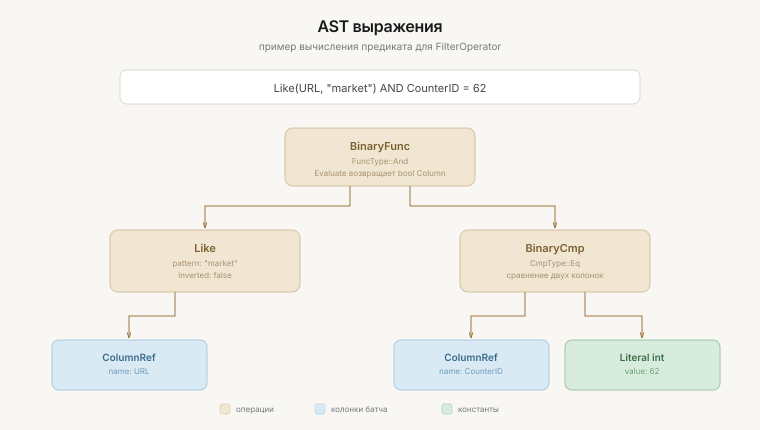
\includegraphics[width=0.9\textwidth]{expression-ast.pdf}
    \caption{Пример AST для выражения \texttt{Like(URL, "market") AND CounterID = 62}.}
    \label{fig:expression_ast}
\end{figure}
\subsubsection{Операторы}
Базовый интерфейс \texttt{IOperator}. Любой оператор должен переопределить методы:

\begin{itemize}
    \item \texttt{std::optional<Batch> Next()} : получить следующий батч.
\end{itemize}

Метод \texttt{Next} реализует pull-based модель исполнения: родительский оператор
для получения результата 
запрашивает данные у своего дочернего оператора. Если данные еще есть,
\texttt{Next} возвращает \texttt{Batch}.
Если входной поток закончился, возвращается \texttt{std::nullopt}.
За счет этого весь план запроса можно собрать как цепочку объектов
\texttt{IOperator}, где каждый оператор хранит указатель на \texttt{child} и вызывает
его \texttt{Next} при необходимости.

Реализованы следующие операторы:

\begin{itemize}
    \item \texttt{ScanOperator} : листовой оператор, читает из \texttt{BZNReader}
    только указанные колонки и возвращает батчи из файла.
    \item \texttt{FilterOperator} : хранит дочерний оператор и предикат
    \texttt{IExpression}. На каждом батче вычисляет предикат, получает булеву маску
    и оставляет только подходящие строки.
    \item \texttt{AggregateOperator} : хранит список агрегаций и выражений,
    вычисляет выражения над входными батчами и накапливает агрегатные состояния без
    группировки.
    \item \texttt{GroupByOperator} : расширяет агрегацию группировкой по ключевым
    выражениям. Для каждого набора ключей хранит отдельные состояния агрегаций. На данный момент группировка производится с помощью \texttt{map<string, state>}.
    Предположим, нужно сделать группировку по колонкам а и б с типами строка и число. 
    В таком случае мы переводим все колонки в строковый тип, склеиваем их через
    разделитель, делаем группировку, на выходе из оператора разбиваем
    строки по разделителю обратно(при этом ключи становятся строками).
    Этот подход самый понятный и простой, за счет этого он является не самым оптимальным
    и проигрывает более оптимальным hash-map. В будущем планируется перейти на сериализацию 
    ключей в единый набор байт и перейти хотя бы на \texttt{std::unordered\_map}.
    \item \texttt{OrderByOperator} : сортирует результат по выражению-ключу.
    Сейчас поддерживается сортировка по одному ключу. Используется \texttt{std::multimap<key, batch>}.
    \item \texttt{OrderByLimitOperator} : поддерживает сортировку с ограничением
    количества строк, то есть top-$k$ по заданному ключу. Реализация такая же как и 
    в \texttt{OrderByOperator}, но в map лежит не больше $k$ элементов за счет чего 
    асимптотика операций становится лучше. От $O(n log n)$ к $O(n log k)$.
    Также выигрываем по памяти от $O(n)$ к $O(k)$ элементов, хранящихся в multimap.
    \item \texttt{LimitOperator} : оставляет первые $k$ строк.
    \item \texttt{OffsetOperator} : пропускает первые $k$ строк.
\end{itemize}

\begin{figure}[ht]
    \centering
    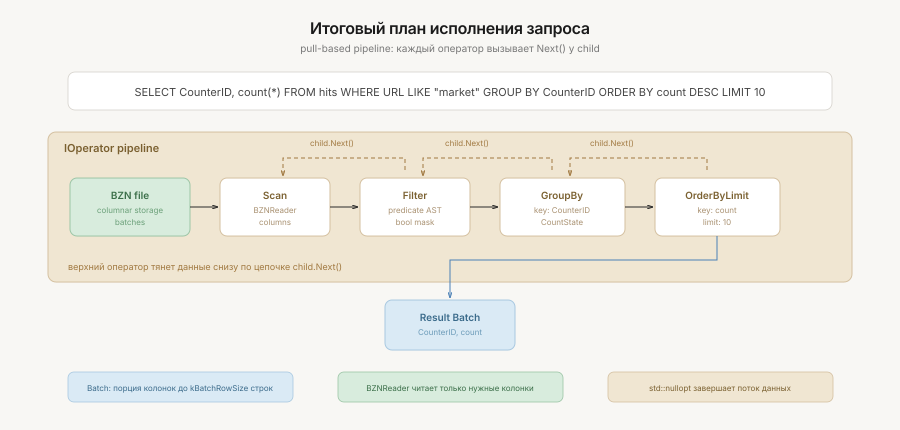
\includegraphics[width=\textwidth]{query-plan.pdf}
    \caption{Итоговый план исполнения запроса в pull-based модели.}
    \label{fig:query_plan}
\end{figure}

\section{Эксперименты}
\subsection{Базовая работа конвертации}

Экспериментальная часть состоит из перекладывания csv файла в колоночный формат и
обратно с различными размерами batch’а (который определяется как количество строк).

Можно обратиться к GitHub \cite{GitHub} и ознакомится с тестами, на которых 
проверяется корректность перевода из одного формата в другой. Таблицы из тестов 
выглядят так:

\begin{table}[ht]
	\caption{schema.csv схема из тестов к таблице ниже}
	\label{table:schema_csv}
	\footnotesize
	\centering
	\begin{tabular}{ll}
		a       & int64  \\
		b       & int64  \\
		name123 & string \\
		d       & int64
	\end{tabular}
\end{table}

\begin{table}[ht]
	\caption{data.csv тестовая таблица для проверки перекладывания данных }
	\label{table:data_csv}
	\footnotesize
	\centering
	\begin{tabular}{llrl}
		1 & 2  & first  & 4 \\
		5 & 1  & second & 2 \\
		8 & 17 & third  & 2
	\end{tabular}
\end{table}

На этих входных данных все корректно перекладывается.



\subsection{Время чтения в зависимости от количества колонок}

Для оценки эффективности селективного чтения колонок был написан отдельный
бенчмарк \texttt{bench\_read\_columns} на базе Google Benchmark. Перед запуском
бенчмарка файл \texttt{hits\_sample.csv} на $999977$ строк был один раз
переложен в \texttt{hits\_sample.bzn}. Далее измерялось полное последовательное
чтение bzn файла с разным количеством выбранных колонок. Между итерациями
производилось загрязнение кэша чтением буфера размером 512 MiB.

Бенчмарк запускался в release сборке. Для каждого случая было выполнено 5
итераций, в таблице указано среднее реальное время одной итерации.


Бенчмарк запускался на железе : chip Apple M4 Pro, 48gb ram, 1tb APPLE SSD AP1024Z. Версия ОС : macOS Tahoe 26.3

\begin{table}[ht]
    \caption{Время чтения bzn файла в зависимости от количества выбранных колонок}
    \label{table:bzn_read_columns_count}
    \footnotesize
    \centering
    \begin{tabular}{rrrr}
        \toprule
        Количество колонок & Строк & Время, мс & Строк/с \\
        \midrule
        1   & 999977 & 1.76    & $1.14 \cdot 10^8$ \\
        2   & 999977 & 2.08    & $9.59 \cdot 10^7$ \\
        4   & 999977 & 1164.70 & $1.72 \cdot 10^5$ \\
        8   & 999977 & 1165.65 & $1.72 \cdot 10^5$ \\
        16  & 999977 & 2738.50 & $7.30 \cdot 10^4$ \\
        32  & 999977 & 2811.55 & $7.11 \cdot 10^4$ \\
        64  & 999977 & 3267.75 & $6.12 \cdot 10^4$ \\
        105 & 999977 & 3531.69 & $5.66 \cdot 10^4$ \\
        \bottomrule
    \end{tabular}
\end{table}

Из таблицы видно, что чтение одной или двух первых колонок выполняется очень
быстро, так как это числовые колонки. При чтении
четырех и более первых колонок в набор попадает строковая колонка \texttt{Title},
которая в текущем формате читается побайтово до разделителя строки. Поэтому
время резко возрастает. Селективное чтение колонок работает,
но строковые колонки являются главным узким местом текущей реализации.

Замер чтения всех колонок одного типа из схемы
\texttt{hits\_scheme.csv}: \texttt{int16}, \texttt{int32}, \texttt{int64} и
\texttt{string}. Колонки типов \texttt{DATE} и \texttt{TIMESTAMP} в этом замере не
учитывались отдельно, достаточно посмотреть на \texttt{int32\_t} и \texttt{int64\_t},
 в bzn формате они физически представлены одинаково.

\begin{table}[ht]
    \caption{Время чтения bzn файла в зависимости от типа выбранных колонок}
    \label{table:bzn_read_columns_type}
    \footnotesize
    \centering
    \begin{tabular}{lrrr}
        \toprule
        Тип колонок & Количество колонок & Время, мс & Строк/с \\
        \midrule
        \texttt{int16}  & 48 & 17.43   & $1.15 \cdot 10^7$ \\
        \texttt{int32}  & 19 & 13.36   & $1.50 \cdot 10^7$ \\
        \texttt{int64}  & 6  & 8.38    & $2.39 \cdot 10^7$ \\
        \texttt{string} & 28 & 3534.03 & $5.66 \cdot 10^4$ \\
        \bottomrule
    \end{tabular}
\end{table}

Результаты подтверждают, что числовые типы читаются существенно быстрее строковых:
они хранятся как непрерывный массив байт и читаются одним блоком. Строки же
сейчас хранятся как последовательность байт с разделителем \texttt{'\textbackslash x1F'}
и читаются посимвольно, что приводит к большому числу операций ввода-вывода и
обработки каждого символа. Хорошим решением будет в дальнейшем хранить строки как
[длина строки][строка], чтобы иметь возможность читать строку блоком.

\subsection{Сравнение с DuckDB}


Условия сравнений такие же как и выше.

\begin{figure}[H]
    \centering
    \includegraphics[width=0.8\textwidth]{../benchmarks/outputs/query_times_comparison.pdf}
    \caption{Сравнение с DuckDB.}
    \label{fig:vsbench}
\end{figure}

N/A -- сравнение недоступно в, реализации отсутствует
 \texttt{ORDER BY} с ключом по больше чем одной колонке и корректная запись пустых батчей,
 что легко доделывается до готового решения.

Рассмотрим запросы, где bzn engine сильно проигрывает DuckDB.

 
\begin{itemize}
    \item Запросы 0, 6, 19 очевидно работают хуже, потому что в случае DuckDB они
    имеют в метаданных min/max/count для каждого батча, что позволяет не
    обновлять состояния и сразу выдавать ответ. Запрос 19 немного выделился на этом фоне,
    так как это не просто агрегация, а сравнение с \texttt{UserId = x}. Благодаря существованию
    min/max можно эффективно пропускать подобные батчи, следовательно, нужно
    меньше чтений.
    \item Сильная разница в запросах 20, 21, 22, 23 31 и 32
    обусловлена не оптимальной реализацией \texttt{groupby}
    а также чтением колонки строкового типа, это место сильно бьет по производительности.
    Даже несмотря на эффективный group by мы проигрываем по причине неэффективного решения
    в bzn формате.
    \item Отсутствует использование многопоточности, есть много мест, которые можно
    оптимизировать используя базовый thread pool, например для пересчета агрегаций
    или \texttt{Like} выражения, где можно, к примеру, разбить колонки на две части, считать
    независимо, после чего просто склеить два ответа вместе.
    \item Отсутствуют simd оптимизации, можно как минимум провести эксперименты с флагами
    компиляции, влияющих на simd и исследовать их влияние на исполнение запросов,
    как максимум проделать большое количество экспериментов с рукописными simd оптимизациями.
    \item Отсутствует работа с размером батча, чем меньше батч, тем больше нужно проводить
    чтений с диска, 
    поиск нужного размера может существенно повлиять на скорость исполнения
    запросов.
\end{itemize}

\section{План совершенствования проекта}

\begin{itemize}
    \item Переход к более сложной логике в \texttt{groupby}, \texttt{map} на строках показывает
     себя очень плохо и тормозит исполнение запросов. Реализация сериализации
     ключей в набор байт и переход в \texttt{hash\_map}.
    \item Улучшение bzn формата. Добавить метаданные
        для колонок, такие как max, min, количество строк в колонке.
        Это позволит эффективно пропускать батчи в запросах вида
        \texttt{SELECT * WHERE UserId = 1337}. Благодаря min/max такое можно будет
        быстро пропускать.
    \item Отсутствует параллелизм и simd оптимизации, есть много не исследованных мест,
    куда это можно добавить и сильно ускорить исполнение.
\end{itemize}

\section{Заключение}
Реализован колоночный формат и конверторы из csv файла в колоночный формат и обратно.
Реализован движок, гибкий к добавлению новой логики
со стороны пользователя и способный проходить большую часть запросов ClickBench.
Пользователь сам строит план запроса.


\newpage
\printbibliography[heading=bibintoc]

\end{document}
